% Deployment chapter continued
\section{Infrastructure from 5,000 feet}
Now, following up from section \ref{infra10k}, the 2nd private subnet is the place where the crawler
resides.
\begin{figure}[h!]
  \centering
  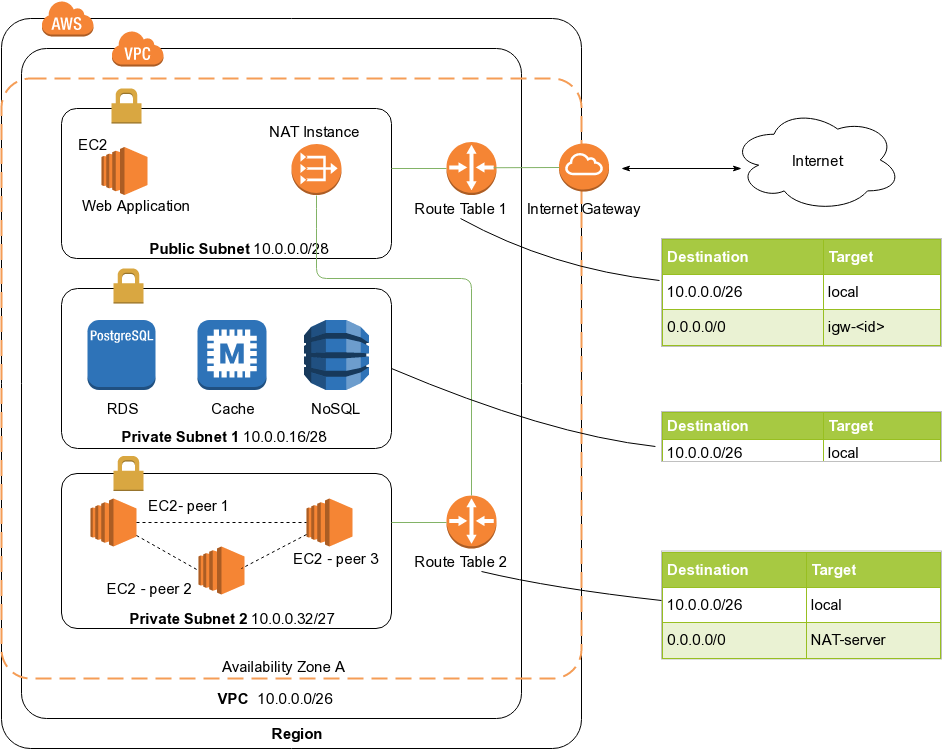
\includegraphics[width=20cm,height=12cm,keepaspectratio]{../media/crawler/aws-deploy-5k-feet.png}
  \caption{Whirlpool infrastructure with Route tables, NAT}
  \label{fig:infra5k}
\end{figure}

\noindent
Each subnet is assigned a default route tables as depicted in figure \ref{fig:infra5k}. NAT instance in public subnet forwards traffic from instances in subnet 2 to the internet and and send the response for corresponding request back to those instances in subnet 2. It won't allow outside clients to initiate connections with instances in subnet 2. The public subnet consists of one application server(EC2) and a NAT instance. The custom route(shown in route table 2)  is created and attached to crawler subnet. The custom rule directs the traffic originated within any of the private subnet peers matching subnet mask \ipAddress{0.0.0.0/0} to NAT server.
\\
\\
At this stage, the public subnet is not really public unless a Internet Gateway(IGW) is attached. After creating a Internet Gateway(IGW), a custom route(show in route table 1) is created and attached to the public subnet. This will scope all packets matching \ipAddress{0.0.0.0/0} route to IGW. The traffic from private
crawler subnet will flow to NAT Instance and then to the IGW. The NAT will translate back-and-forth source
and destination IPs of private instances.
\\
\\
The data store private subnet contains RDS instance(PostgreSQL as part of the implementation). The
extracted data is persisted in MongoDB which is a NoSQL variant. AWS does not have managed instance of
MongoDB and requires the interested party to operate, maintain on an EC2 Instance. Finally, to improve
lookup time efficiency of few subsystems within the whirlpool, AWS ElasticCache is leveraged. 

% note - here expand on EC2, RDS, cache, NoSQL, NAT computing specifications
\section{AWS Services Hardware Specfication \& Cost Estimation}

\begin{figure}[h!]
  \centering
  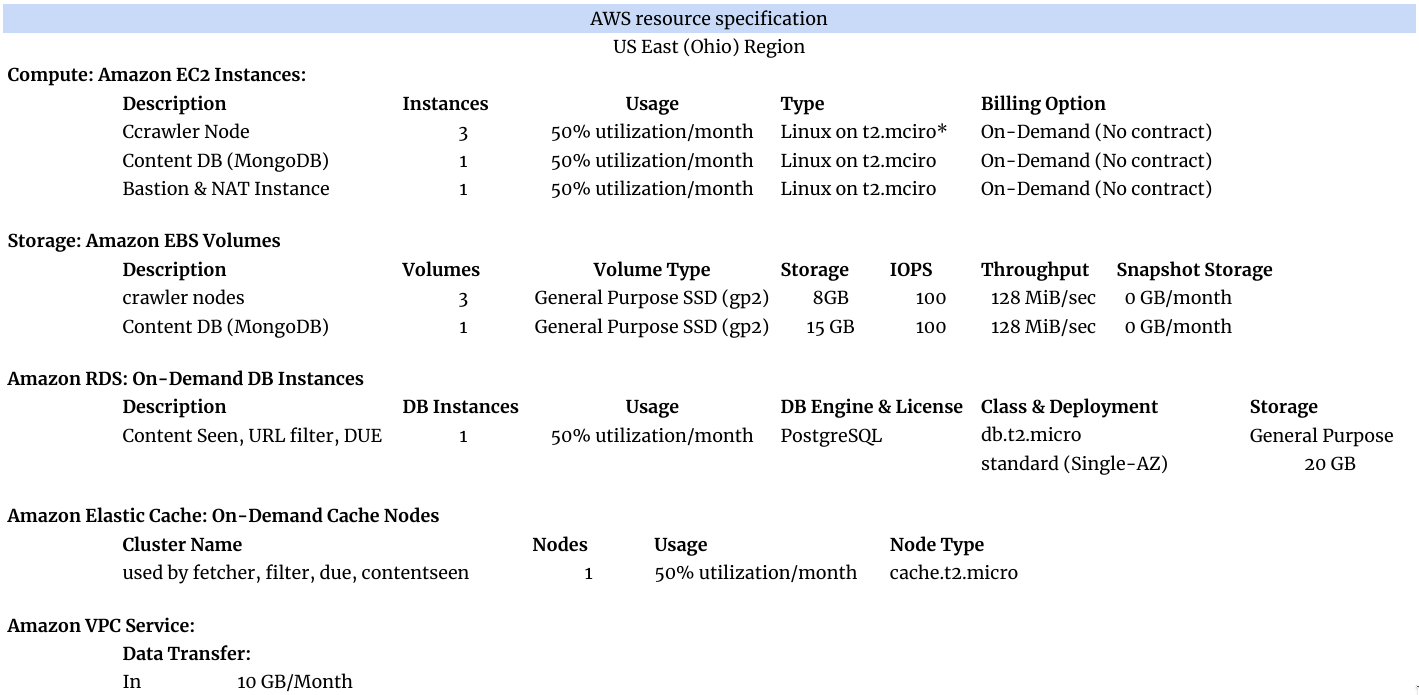
\includegraphics[width=16cm,height=13cm,keepaspectratio]{../media/crawler/aws-resource.png}
  \caption{Whirlpool Hardware Specification on AWS}
  \label{fig:awsspec}
\end{figure}

\noindent
From table \ref{fig:awsspec} under Amazon EC2 services, a crawler node sits on a on-demand EC2 instance which is of type t2.micro. The t2.micro has single core virtual CPU (vCPU) with 1 GiB of Memory. Each crawler node runs a message broker - RabbitMQ to interconnect the crawler subsystems. According to RabbitMQ Documentation
\cite{rabbitmq}, the host should have at least 128 MB memory available at all times. Moreover, it wont accept
any new messages when it detects that its using more than 40\% of avialable memory. Being said that, there is
always an option to change the current instance type from t2.micro to t2.small and so on depending on
usage. MongoDB which collects extracted text is hosted on On-Demand t3.micro instance type, which is a 1 GB, dual-core vCPU operating at 50\% of its capacity.
\\
\\
\noindent
Coming to Amazon Storage,  the crawler node is coupled with Elastic Block Storage(EBS) volume of 5 GB. The volume is general purpose SSD capped at 100 IOPS giving a throughput of 128 MB/sec. For mongoDB an EBS volume
of 15GB is used. It is formatted with XFS filesystem for its data directory as recommended in its production checklist.
\\
\\
\noindent
Whirlpool uses one On-Demand RDS instance with PostgreSQL engine operating at 50\% utilization monthly. The underline managed Operating System is a db.t2.micro deployed in a single AZ. PostgreSQL to store fingerprints of a web page content at a given URL, robots.txt attributes of each site, and URLs already enqueued to be crawled.
\\
\\
Amazon ElasticCache provides a choice between Memcached \& Redis Instance. It will be used by URL filter
subsystem of whirlpool.
\\
\\
Lastly, Amazon VPC has a NAT Gateway which will process data estimated close to 10 GB/month. Regardless of data flow inward/outward, the NAT is charged by the hour.
\\
\\
\noindent
Table \ref{fig:awscost} provides approximate monthly billing information of AWS services used by this project to build, test, and run experiments. The calculation was performed using AWS monthly calculator. At the time of this writing, the author is enrolled is 12-month AWS Free tier access which discounts most of the services
the crawler system leverages.

\begin{figure}[h!]
  \centering
  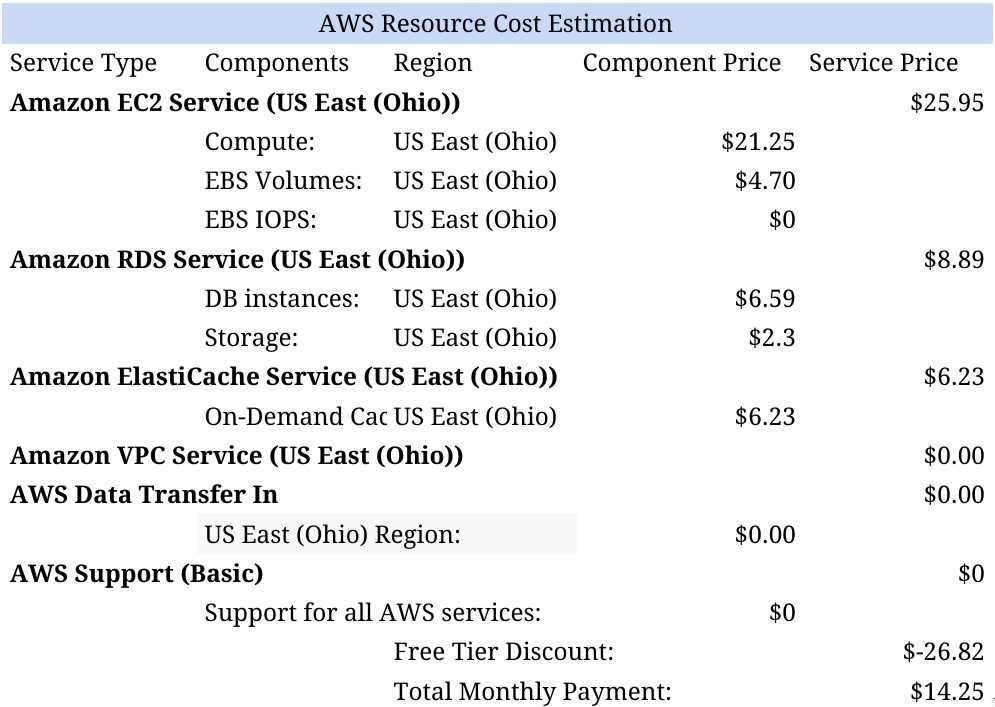
\includegraphics[width=12cm,height=8cm,keepaspectratio]{../media/crawler/aws-resource-cost-estimation.png}
  \caption{Whirlpool Hardware Cost Estimation on AWS}
  \label{fig:awscost}
\end{figure}

\noindent
With the free-tier in use, the total price is dropped almost by 50 \%. Under free tier, EC2 is limited to 750 hours/month which equates to approx. 24 hours/day for 30 days using only Linux, RHEL. Any combination of EBS (SSD/Magnetic) is 30 GiB. Amazon RDS again limited to 750 hours/month upto 20GB of general purpose SSD database
storage. Amazon ElasticCache - 750 hours. NAT Gateway is charged \dollar{0.045} an hour. There is no charge for data transfer between cross-region multi-AZ as this implementation is 1 region, single AZ. Also, the data 
transfer into AWS cloud is free.

\pagebreak